\question{Насыщение перехода}

\begin{figure}[h!]
	\center
	\vspace{-2em}
	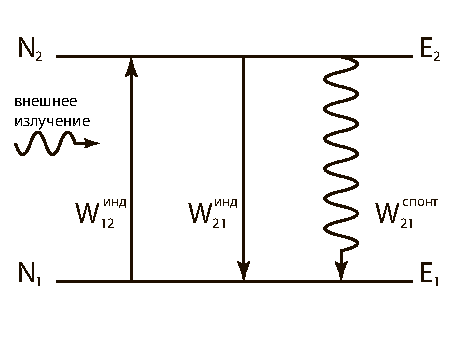
\includegraphics[width=.4\textwidth]{06_01}
	\vspace{-2em}
\end{figure}

Скорость заселения верхнего уровня
\[
    \der{N_2}{t} = W^\text{и}_{12} N_1 - W^\text{и}_{21} N_2 - 
    W^\text{сп}_{21} N_2.
\]

Под насыщенным переходом внешнего излучения понимается зависимость 
коэффициента поглощения слабого сигнала при воздействии на среду внешним 
излучением. Выясним, от чего зависит \( \D N = N_2 - N_1 \).

Изменение интенсивности проходящего через среду света с одной стороны равно
\( dI = -\alpha I dx \), с другой~-- \( dI = W_{12}(n_2 - n_1 ) h\nu dx \).

Поскольку \( B_{12} = B_{21} \), то \( W^\text{и}_{12} = W^\text{и}_{21} = W \).
Вероятность спонтанного излучения \( W^\text{сп}_{21} = A_{21} = 1 / \tau \).
Тогда
\[
    \der{N_2}{t} = WN_1 - WN_2 - \frac{N_2}{\tau}; \quad
    \der{N_2}{t} = -W\D N - \frac{N_2}{\tau}.
\]
Общая заселенность уровней \( N = N_2 + N_1 \).
Учитывая, что \( N + \D N = 2N_2 \), получим
\[
    \der{}{t}\left( \frac{\D N}{2} + \frac{N}{2} \right) = -W\D N - 
    \frac{\D N}{2\tau} - \frac{N}{2\tau}.
\]

Рассмотрим квазистационарный случай: \( \D N = const \), тогда
\( d(\D N) / dt = 0 \). Получим:
\[
    -\D N\left( 2W + \frac{1}{\tau} \right) - \frac{N}{\tau} = 0, \quad
    \text{ или } \quad \D N = \frac{-N}{1 + 2W\tau}.
\]

Таким образом, разность населённостей энергетических уровней зависит от:
\begin{enumerate}
  \item времени жизни в возбужденном состоянии \( \tau \),
  \item от объёмной плотности воздействующего на систему внешнего
    электромагнитного поля, изменяющего вероятности индуцированных переходов
    \( W \).
\end{enumerate}
